\chapter{Project Requirement Analysis}\label{ch:ProjectRequirementAnalysis}
\section{Architectural Description}\label{sec:ArchitecturalDescription}
Client-Server Architecture: Our system will adopt a client-server model, which consists of multiple clients interfacing with a cluster of server nodes. The clients are responsible for querying current stock levels and submitting updates for processing. The server nodes serve these stock level requests and manage inventory updates. Amongst the server nodes, a leader will be elected to coordinate updates and ensure consistency across the distributed system.


\section{Dynamic Discovery of Hosts}\label{sec:DynamicDiscoveryOfHosts}
Server-side: Upon initiation, each server node will broadcast its presence and listen for existing members of the system to construct a current view of the cluster. The broadcast message from the joining server is only responded by the
leader of the system. The message contains an array with all ip addresses currently active within the system, as well as the information which node is the leader.

When the servers are started, no leader is chosen at this point of time. In this case, the first node which does not get a reply of his broadcast declares himself as leader and answers the requests of the other nodes.
To ensure, that only one leader is chosen at the starting point, a random sleep is implemented, which ensures the existence of only one leader.

This dynamic discovery protocol allows the system to scale horizontally without manual configuration.

Client-side: Clients are designed to automatically detect server nodes in the system. As well as the server-side implementation a broadcast message is sent, but not with the intention
to join the cluster. In the Client-side case the ip address is not added to the server node pool. The reply to the broadcast is done by the leader, sending an array of all members to the client. 
The client uses one randomly chosen address to communicate with. If the reply of an request by an client is not answered by the node, another discovery will be done to get an updatet version of the list with nodes.

This enables seamless interaction with the inventory system, ensuring that clients can always locate a server node to process their requests.

\section{Fault Tolerance}\label{sec:FaultTolerance}
Our system is engineered to handle different types of failures, ensuring continuous operation:
Leader Failure: If the current leader server fails, the remaining servers will initiate a leader election to select a new leader. In the meantime no operation is permitted, because our system uses strong consistency. As soon as a new leader is elected, the system returns to normal process.
This ensures that the system become available after a crash of the leader.

Server Crash: In the event of a server crash, client requests are automatically redirected to other operational server nodes. A health check mechanism and a server list update protocol ensure that clients and servers are aware of the available nodes in real-time. When a node does not send a Heartbeat,
it will be removed from the list by every server, including the leader, so the normal processing can continue.

Retry Logic: To handle transient failures, the system will implement a retry mechanism. This ensures that, for instance, during a purchase processing, if a write operation fails, the system will retry the operation. We will have a limit to  prevent excessive retries that could overwhelm the system, allowing it to fail and recover.

\section{Leader Election}\label{sec:Election}
Consensus on Updates: Write operations, critical for inventory synchronisation, are managed by the leader node. Also new nodes which want to join the group exchange information with the leader. The election Algorithm will be the bully Algorithm.
When an election is triggered (the heartbeat of the leader is missing), the first Server, which realises it, starts an election, using an ID as information multicastet to every other server. If another Server has an higher id, he claims to become the leader,
\enquote{bullying} the server with a lower ID and denying his election. This will continue unitl the server with the highest ID wins the election. He then sends a message, declaring himself as new leader and the workflow can continue.

\section{Ordered Reliable Multicast}\label{sec:OrderedReliableMulticast}
Our system uses total ordered reliable multicast to ensure inventory updates, like purchases or deletions, are processed sequentially, maintaining data consistency and preventing access to outdated item statuses. In the ordered reliable multicast the leader acts as the sequencer. All messages are sent to the leader, the leader then sends the messages to all hosts via udp multicast. Each message contains a sequence number and the actual content. When a host receives a message from the leader the message is put into the log and an acknowledge is sent to the leader. As we strive for full consistency the leader wait's until it received an acknowledge from all active hosts. After receiveing all acknowledgements the leader sends a commit message to all hosts triggering that the messag is processed. In case a host recieves a messag with a sequence number which is bigger than his sequence number + 1 it requests from the leader all messages starting from it's current sequence number up to the received sequence number. By this it's guaranteed that each host maitains the same state. 




\begin{figure}[h!]
        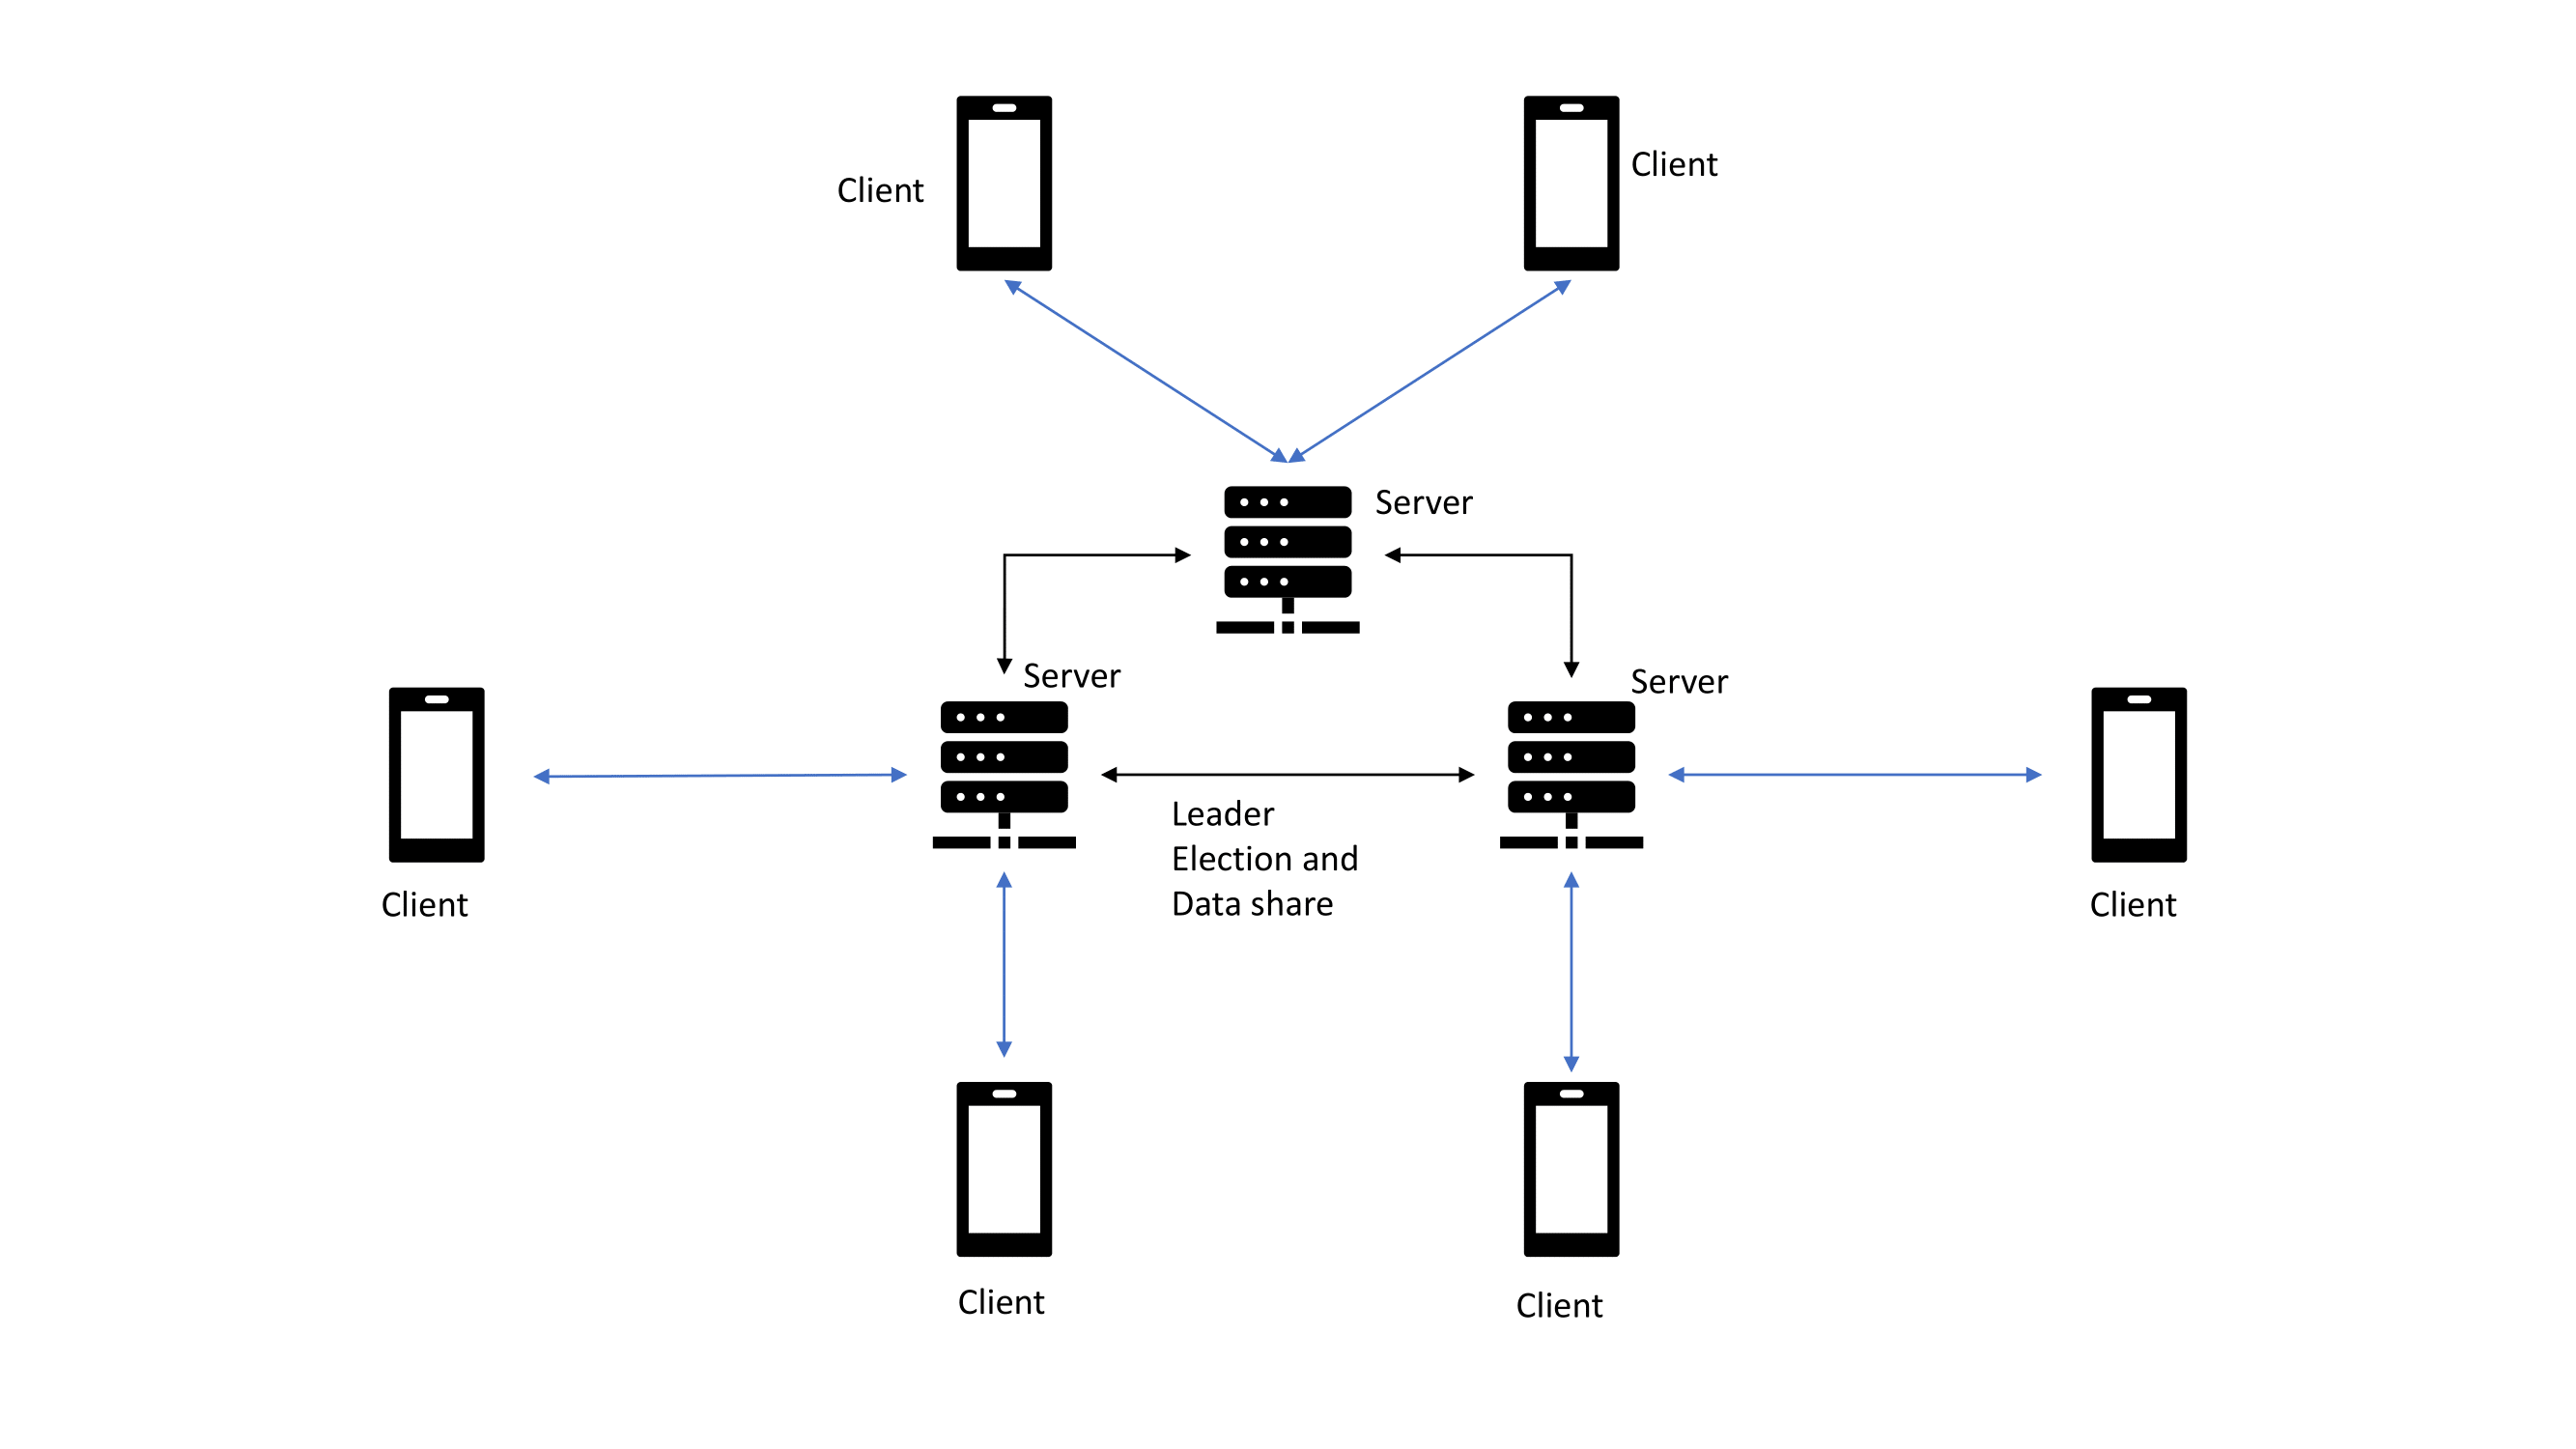
\includegraphics[height=10cm, width=18cm]{images/Architecture.png}
        \caption{Architecture Diagram}
        \label{fig:architecture}
\end{figure}
